\documentclass[a4paper,12pt]{article}

\usepackage[T1]{fontenc}
\usepackage[absolute]{textpos}
\usepackage[latin1]{inputenc}
\usepackage[document]{ragged2e}
\usepackage{amsmath}
\usepackage{graphicx}
\usepackage{setspace}
\usepackage{xcolor}
\usepackage{soul}
\usepackage{fancyhdr}
\usepackage{pgf-pie}   
\usepackage{pgfplots}
\usepackage{listings}


\graphicspath{ {images/} }
\setlength{\TPHorizModule}{1cm}
\setlength{\TPVertModule}{1cm}

\title{\textbf{\Huge Analizador L�xico}}
\date{}

\renewcommand{\headrulewidth}{0pt}
\doublespacing

\pagestyle{fancy}
\fancyhf{}
\rfoot{\thepage}
\fancyhead[L]{\emph{\rightmark}}

\renewcommand*\contentsname{�ndice}

\definecolor{MoradoChogath}{rgb}{0.42,0.08,0.78}
\definecolor{Black}{rgb}{0,0,0}
\definecolor{LBlue}{rgb}{0.14,0.43,0.89}
\definecolor{LRed}{rgb}{0.89,0.14,0.30}
\definecolor{LOrange}{rgb}{0.90,0.38,0.15}

\definecolor{PGreen}{rgb}{0.19,0.86,0.45}
\definecolor{DBlue}{rgb}{0.16,0.19,0.76}
\definecolor{PYellow}{rgb}{1,0.81,0.33}
\definecolor{PBlue}{rgb}{0.29,0.55,0.70}
\definecolor{PPGreen}{rgb}{0.31,0.79,0.55}
\definecolor{DGray}{rgb}{0.33,0.33,0.33}
\definecolor{DPumpkin}{rgb}{0.80,0.48,0.4}
\definecolor{MGreen}{rgb}{0.12,0.82,0.1}


%Color de resaltado%
\sethlcolor{LRed}

\pgfplotsset{width=14cm,compat=1.9}
\lstset{
    escapeinside={(*@}{@*)},
	basicstyle=\sffamily\footnotesize,
}

\begin{document}
	\begin{titlepage}
	\centering
			\begin{textblock}{5}(3.5,2)
				
\includegraphics[width =14cm, height=3cm]{ulogo}
			\end{textblock}
			\maketitle
			\thispagestyle{empty}



			{\Large\text{\textbf{Profesor:}}\\}
			\begin{large}	
				\text{Ing. Sleyter Angulo}\\
			\end{large}
			{\Large\text{\textbf{Proyecto II}}\\}
			
			{\large\text{Estructura de datos II BISOFT-28}\\}
			{\large\text{\emph{Ingenier�a del software}}\\}			

			{\Large\text{\textbf{Integrantes:}}\\}
			\begin{large}	
				\text{Jes� Abraham Ch�vez} \\
				\text{Daniel Hernandez Sanchez} \\
				\text{}\\
				\text{}\\
				\text{}\\
				\text{\textbf{III Cuatrimestre 2021}} \\
			\end{large}
	\end{titlepage}

	\clearpage

	\setcounter{page}{1}

	\tableofcontents

	\newpage 
	\section {Scanner}
	\setlength{\parindent}{1,5cm}
	\subsection{Proceso de scanning}
	\justify 
	El proceso de scanning, tambi�n conocido como an�lisis l�xico, es la primera fase del proceso de compilaci�n. 

	�ste es  realizado por un Scanner o analizador l�xico, que en l�neas generales, se trata de un programa que recibe a modo de entrada el c�digo fuente de otro, y a partir de las secuencias de caracteres contenidas en �ste, genera una serie de tokens, cuyo ciclo de vida continua en un analizador sint�ctico o Parser. 

	Cada token generado por el Scanner representa un componente l�xico o s�mbolo, cuyo patr�n es detectado mediante expresiones regulares. Dichas expresiones pueden ajustarse seg�n los requerimientos del lenguaje con el que se est� tratando.  

	Las expresiones regulares que definen los tokens del lenguaje son revisadas por un aut�mata de estados finitos, encargado de  procesar car�cter a car�cter el c�digo fuente pasado como entrada, y retornar un token por cada estado final alcanzado.

	En el caso de que existan m�s de dos patrones en los que una secuencia de caracteres pueda alcanzar un estado final, se toma la que mayor cantidad de coincidencias individuales posea.

	El proceso de scanning implementado en este proyecto no se separa del proceso descrito anteriormente, al menos no en el orden y objetivo de cada paso a realizar. 
	
	\newpage
	Apoyados en la herramienta Flex, - de la que se hablar� con mayor detalle m�s adelante -, y en un conjunto de expresiones regulares que representan al lenguaje de programaci�n Pascal, generamos un aut�mata de estados finitos en C++, que retorna los tokens a otro programa escrito en el mismo lenguaje, cuyo trabajo es la realizaci�n de este documento.
	
	Ambos programas utilizan el archivo de cabecera Token.h, que contiene una colecci�n de tipos de token, as� como la forma de tratarlos al momento de ser representados en la salida.
	
	\begin{center}
		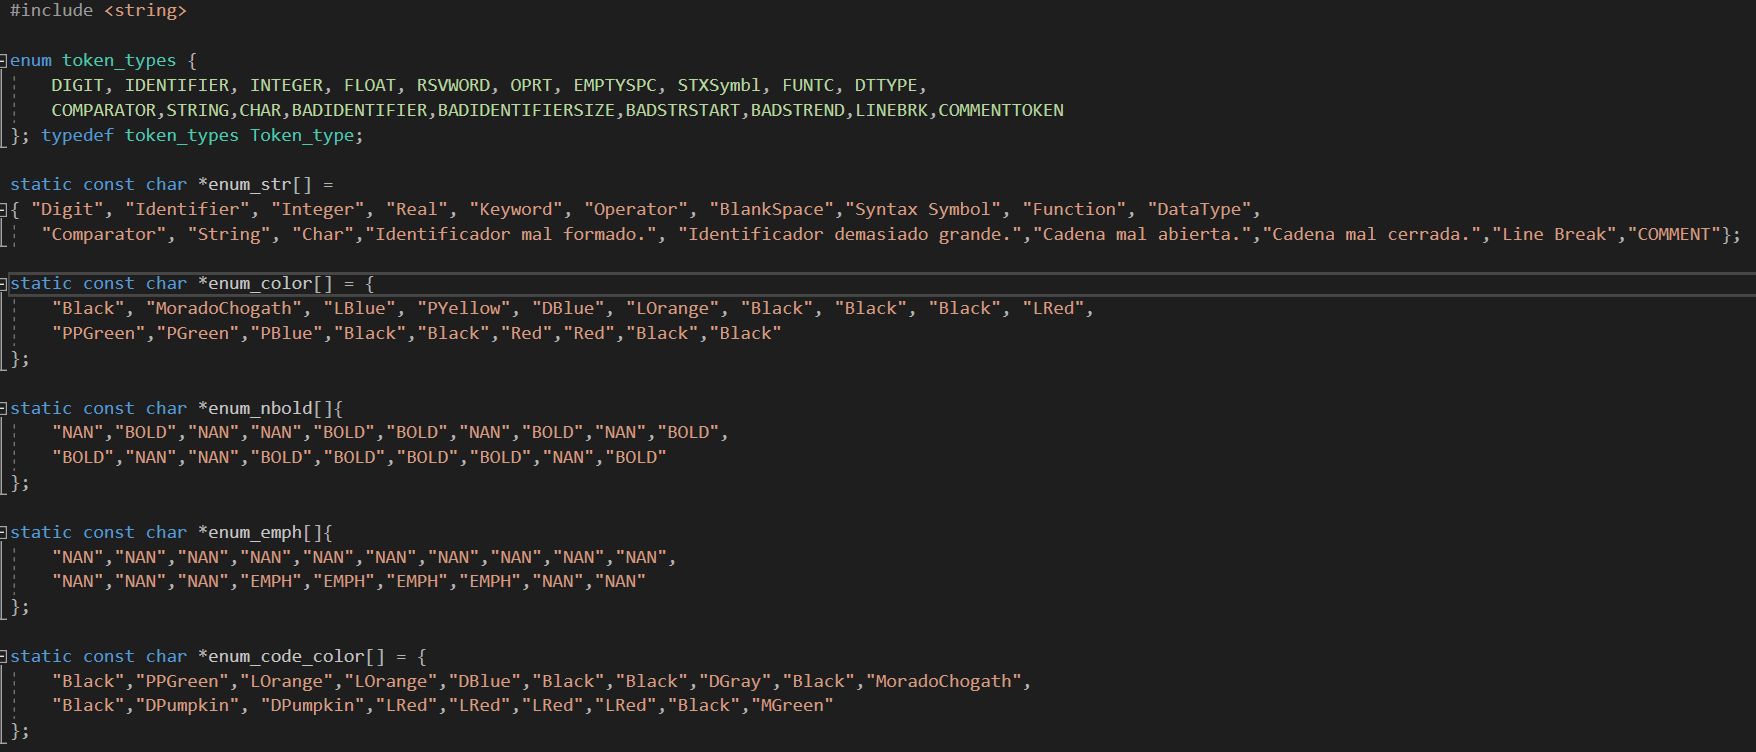
\includegraphics[width =14cm, height=10cm]{tokenh}
	\end{center}
	
	\newpage
	Los tokens son almacenados en la siguiente estructura:
	\begin{center}
		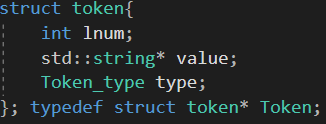
\includegraphics[width =6cm, height=3cm]{structtoken}
	\end{center}

	Cada token detectado se almacena en una cola que servir� para recomponer el c�digo fuente en la secci�n correspondiente de este documento.

	\newpage 
	\setlength{\parindent}{1,5cm}
	\subsection{Flex}
	Flex es un software open source desarrollado alrededor del a�o 1987 por Vern Paxson en el lenguaje C. Flex significa Fast Lexical analyzer generator y como el nombre lo menciona, esta herramienta nos permite realizar y generar un analizador l�xico para diversos prop�sitos, a estos analizadores l�xicos se les denomina "Scanners" o "Lexers".  Para su complementar su funcionalidad, esta herramienta se puede llegar a utilizar junto con Berkeley Yacc Parsser Generator � GNU Bison parser generator, ambos siendo software para el an�lisis de texto. 
	
	Con la herramienta Flex, podemos generar un analizador l�xico para cualquier lenguaje en corto tiempo, ya que a este solo se le deben de indicar los patrones a buscar, las reglas al reconocer los patrones y las acciones que se deben tomar una vez encontrados. Flex genera un archivo .l el cual contiene todas las reglas definidas por el programador. Dentro de los archivos generados, se crea una funci�n  yylex(), la cual es la responsable por ejecutar el archivo .l para comenzar a leer el documento pasado por par�metros y comenzar a reconocer y devolver los tokens encontrados.  


	\newpage 
	\section {Resultados}	
	\subsection{C�digo escaneado}
	\begin{lstlisting}

(*@\textcolor{DBlue}{\textbf{Program}}@*) (*@\textcolor{PPGreen}{\textbf{ejb}}@*)(*@\textcolor{DGray}{\textbf{;}}@*)
(*@\textcolor{DBlue}{\textbf{uses}}@*) (*@\textcolor{PPGreen}{\textbf{crt}}@*)(*@\textcolor{DGray}{\textbf{;}}@*)
	(*@\textcolor{DBlue}{\textbf{Var}}@*)
		(*@\textcolor{PPGreen}{\textbf{R}}@*)(*@\textcolor{DGray}{\textbf{,}}@*)(*@\textcolor{PPGreen}{\textbf{Num1}}@*)(*@\textcolor{DGray}{\textbf{,}}@*)(*@\textcolor{PPGreen}{\textbf{num2}}@*)(*@\textbf{:}@*)(*@\textcolor{MoradoChogath}{\textbf{integer}}@*)(*@\textcolor{DGray}{\textbf{;}}@*)

(*@\textcolor{DBlue}{\textbf{Begin}}@*)
(*@\textcolor{PPGreen}{\textbf{clrscr}}@*)(*@\textcolor{DGray}{\textbf{;}}@*)
	(*@\textcolor{DBlue}{\textbf{Writeln}}@*)(*@\textcolor{DGray}{\textbf{(}}@*)(*@\textcolor{DPumpkin}{'Ingrese\phantom{x}Un\phantom{x}numero'}@*)(*@\textcolor{DGray}{\textbf{)}}@*)(*@\textcolor{DGray}{\textbf{;}}@*)
	(*@\textcolor{DBlue}{\textbf{Readln}}@*)(*@\textcolor{DGray}{\textbf{(}}@*)(*@\textcolor{PPGreen}{\textbf{Num1}}@*)(*@\textcolor{DGray}{\textbf{)}}@*)(*@\textcolor{DGray}{\textbf{;}}@*)
	(*@\textcolor{DBlue}{\textbf{Writeln}}@*)(*@\textcolor{DGray}{\textbf{(}}@*)(*@\textcolor{DPumpkin}{'Ingrese\phantom{x}Un\phantom{x}numero'}@*)(*@\textcolor{DGray}{\textbf{)}}@*)(*@\textcolor{DGray}{\textbf{;}}@*)
	(*@\textcolor{DBlue}{\textbf{Readln}}@*)(*@\textcolor{DGray}{\textbf{(}}@*)(*@\textcolor{PPGreen}{\textbf{Num2}}@*)(*@\textcolor{DGray}{\textbf{)}}@*)(*@\textcolor{DGray}{\textbf{;}}@*)
	(*@\textcolor{PPGreen}{\textbf{R}}@*)(*@\textbf{:=}@*)(*@\textcolor{PPGreen}{\textbf{Num1}}@*)(*@\textbf{-}@*)(*@\textcolor{PPGreen}{\textbf{Num2}}@*)(*@\textcolor{DGray}{\textbf{;}}@*)
	(*@\textcolor{DBlue}{\textbf{Writeln}}@*)(*@\textcolor{DGray}{\textbf{(}}@*)(*@\textcolor{DPumpkin}{'Al\phantom{x}restar:\phantom{x}'}@*)(*@\textcolor{DGray}{\textbf{,}}@*) (*@\textcolor{PPGreen}{\textbf{num1}}@*)(*@\textcolor{DGray}{\textbf{,}}@*)(*@\textcolor{DPumpkin}{'\phantom{x}-\phantom{x}'}@*)(*@\textcolor{DGray}{\textbf{,}}@*)(*@\textcolor{PPGreen}{\textbf{num2}}@*)(*@\textcolor{DGray}{\textbf{,}}@*)(*@\textcolor{DPumpkin}{'\phantom{x}se\phantom{x}obtiene:\phantom{x}'}@*)(*@\textcolor{DGray}{\textbf{,}}@*)(*@\textcolor{PPGreen}{\textbf{R}}@*)(*@\textcolor{DGray}{\textbf{)}}@*)(*@\textcolor{DGray}{\textbf{;}}@*)
(*@\textcolor{DBlue}{\textbf{readln}}@*)(*@\textcolor{DGray}{\textbf{;}}@*)
(*@\textcolor{DBlue}{\textbf{ENd}}@*)

Errores encontrados: 


 \end{lstlisting}
	\newpage 
	\subsection{Histograma}	

	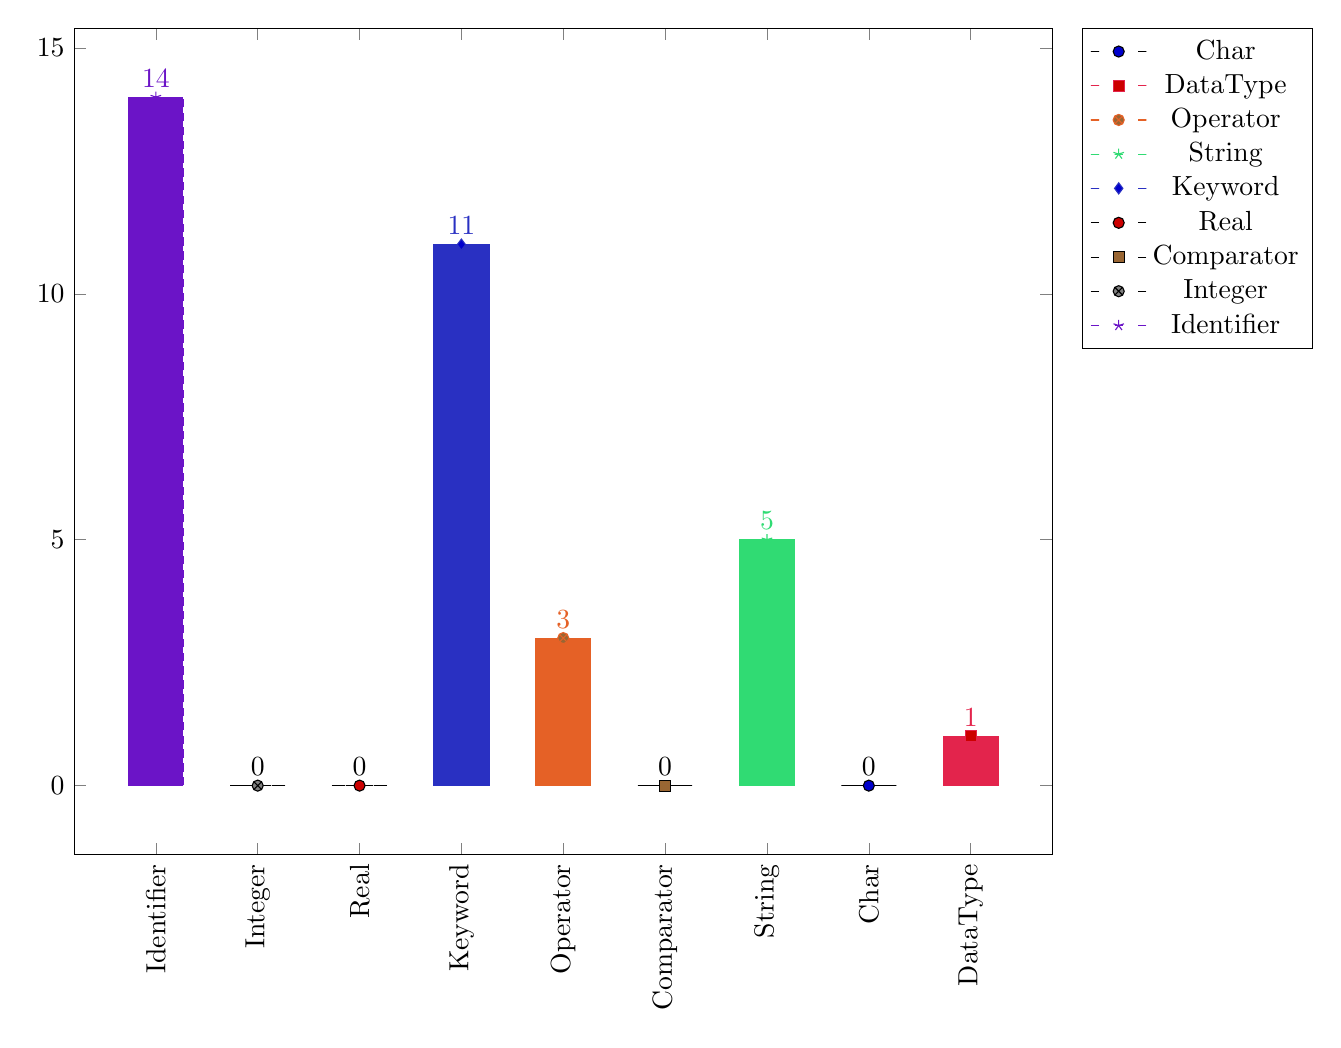
\begin{tikzpicture}
	\begin{axis}[
			legend pos=outer north east,  %-- Colocacion de la leyenda en la parte superior derecha del grafico%
			%legend style={draw=none,at={(0.5,-0.15)}, text width=2.5cm,%
			%anchor=north,legend columns=-1},	 Colocacion de la leyenda en la parte inferior del grafico%		
			axis on top,
			bar width = 0.7cm,
			xticklabel=\empty,
		    ytick distance=5,
			nodes near coords,
		    xtick distance=1,
			xticklabel style={rotate=90},
			every axis plot/.append style={
			  ybar,
			  bar shift=0pt,
			  fill
			},
symbolic x coords = {Identifier,Integer,Real,Keyword,Operator,Comparator,String,Char,DataType}]\addplot+[Black] coordinates{(Char,0)}; 
\addplot+[LRed] coordinates{(DataType,1)}; 
\addplot+[LOrange] coordinates{(Operator,3)}; 
\addplot+[PGreen] coordinates{(String,5)}; 
\addplot+[DBlue] coordinates{(Keyword,11)}; 
\addplot+[Black] coordinates{(Real,0)}; 
\addplot+[Black] coordinates{(Comparator,0)}; 
\addplot+[Black] coordinates{(Integer,0)}; 
\addplot+[MoradoChogath] coordinates{(Identifier,14)}; 
\legend{Char,DataType,Operator,String,Keyword,Real,Comparator,Integer,Identifier} 
\end{axis} 
	\end{tikzpicture}	\newpage 
										\subsection{Diagrama circular}
										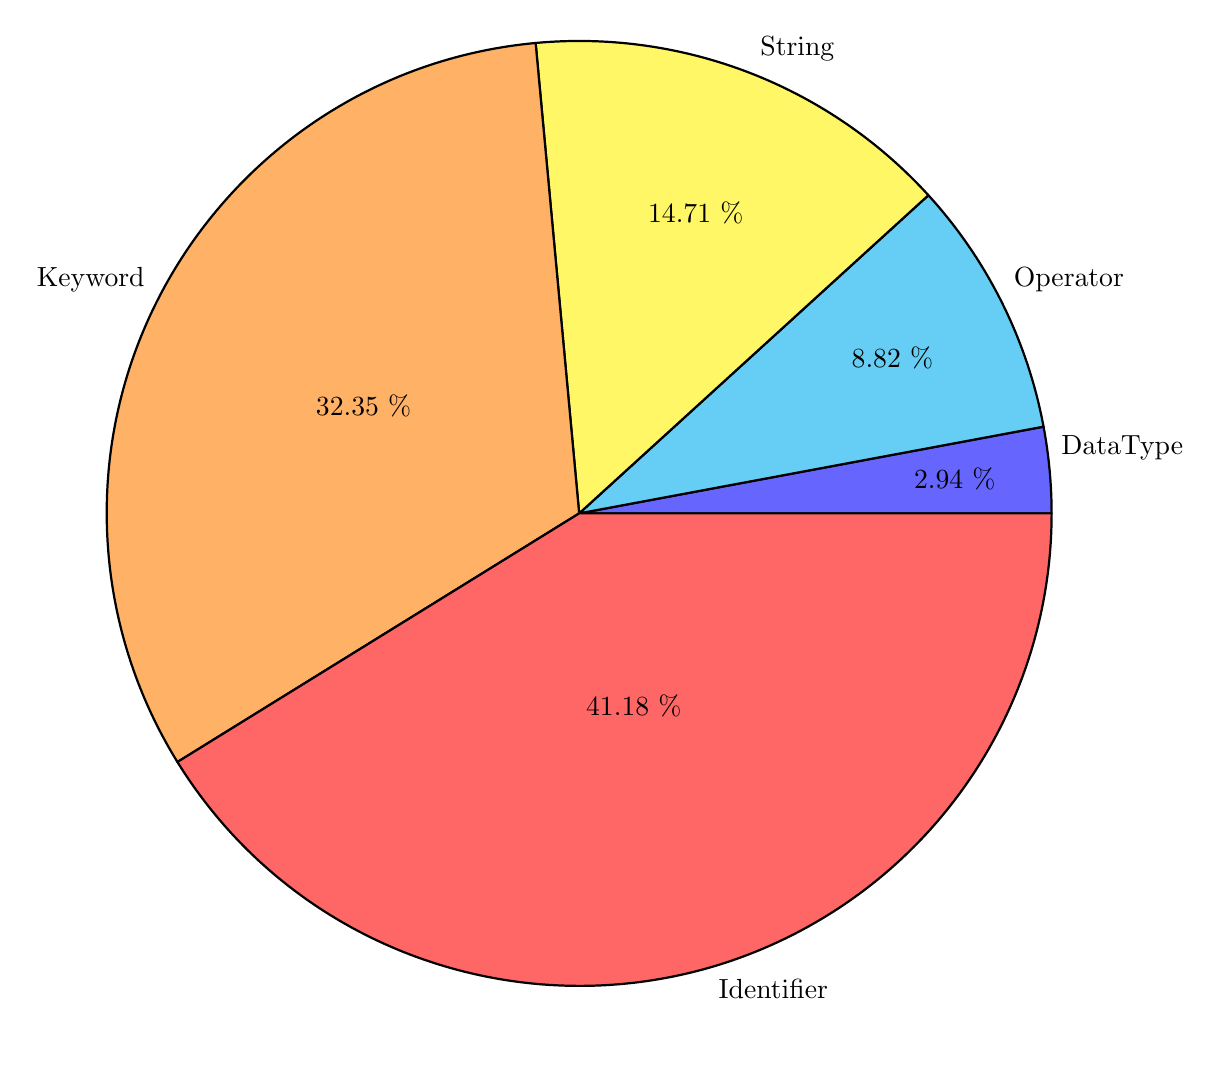
\begin{tikzpicture}

 \def\printonlypositive#1{\ifdim#1pt>0pt 
 #1 
 \fi} \pie[xshift=12cm,scale=2,before number=\printonlypositive]{2.94/DataType,
8.82/Operator,
14.71/String,
32.35/Keyword,
41.18/Identifier
}
 \end{tikzpicture}
\end{document}